% Szglab4
% ===========================================================================
%
\chapter{Szkeleton tervezése}

\thispagestyle{fancy}

\section{A szkeleton modell valóságos use-case-ei}

\subsection{Use-case diagram}

\begin{figure}[h]
\begin{center}
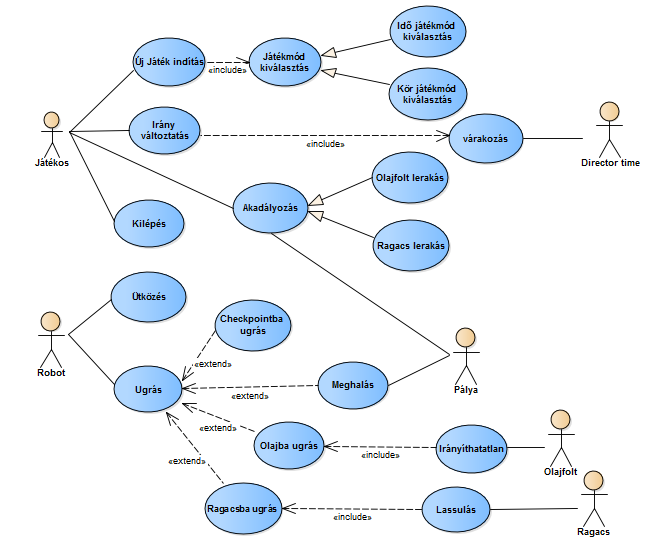
\includegraphics[width=17cm]{skeleton_use_case3.PNG}
\caption{Use-case diagramm}
\label{fig:SzkeletonUseCase}
\end{center}
\end{figure}
\newpage

\subsection{Use-case leírások}

\usecase{Új játék indítása}
{A játékos elindítja a játékot.}
{Játékos}
{A grafikus felületen (menüben) a felhasználó rákattinthat az „Új Játék indítása” menüpontra.}

\usecase{Játékmód kiválasztás}
{Választás a játékmódok közül}
{Játékos}
{A játékos tud választani két játékmód közül, hogy milyen játékmódban szeretne játszani.}

\usecase{Idő játékmód kiválasztása}
{A játékos kiválasztja az idő játékmódot.}
{Játékos}
{A grafikus felületen (menüben) a felhasználó olyan játékmódban indítja el a játékot amiben egy számláló fut visszafelé, és ha lejár, vége a játéknak.}

\usecase{Kör játékmód kiválasztása}
{A játékos kiválasztja a kör játékmódot.}
{Játékos}
{A grafikus felületen (menüben) a felhasználó olyan játékmódban indítja el a játékot, melyben el kell érni egy megadott körszámot, és ezután ér véget a játék.}

\usecase{Irányváltoztatás}
{A robot irányának beállítása.}
{Játékos}
{A robot ugrása előtt lehetőség van beállítani az irányát 3 másodpercig.}

\usecase{Várakozás}
{Egy számláló 3 másodpercig visszaszámol.}
{Director time}
{A körökre osztás miatt a robot csak három másodpercenként ugrik.}
\pagebreak

\usecase{Akadályozás}
{A pályára akadályok kerülnek.}
{Játékos, Pálya}
{A játékos utasíthatja a robotot, hogy rakjon le akadályt a pályára, illetve a pályára is kerülnek akadályok a játék elején.}

\usecase{Olajfolt lerakás}
{A pályára olajfolt kerül.}
{Játékos}
{A robot olajfoltot rak le a pályára a játékos utasítására.}

\usecase{Ragacs lerakás}
{A pályára ragacs kerül.}
{Játékos}
{A robot ragacsot rak le a pályára a játékos utasítására.}

\usecase{Kilépés}
{A játékos kilép a játékból.}
{Játékos}
{A felhasználó visszalép a menübe, vagy teljesen leállítja a játék működését.}

\usecase{Ütközés}
{Robotok ütköznek}
{Robot}
{Két robot összeütközése után lepattannak egymásról.}

\usecase{Ugrás}
{A robot ugrik a megadott irányba.}
{Robot}
{A játékos a megadott billentyűkkel beállítja az ugrás irányát, majd a robot ugrik.}
\newpage

\usecase{Checkpointba ugrás}
{A robot beleugrik egy checkpointba.}
{Robot}
{A robot körmegtételének ellenőrzése miatt a robotnak checkpointokba kell beleugrálnia.}

\usecase{Meghalás}
{A robot meghal.}
{Pálya}
{Az ugrás után, ha a robot nem tartózkodik a pályán, akkor meghal.}

\usecase{Olajba ugrás}
{A játékos olajfoltba ugrik.}
{Robot}
{A robot az ugrás után egy olajfoltra érkezik a pályán.}

\usecase{Irányíthatatlan}
{A robot irányíthatatlan lesz.}
{Olajfolt}
{A játékos nem fogja tudni megváltoztatni a következő körben a robot ugrásának irányát, az „csúszni” fog tovább.}

\usecase{Ragacsba ugrás}
{A játékos ragacsba ugrik.}
{Robot}
{A robot az ugrás után egy ragacsba érkezik a pályán.}

\usecase{Lassulás}
{A robot sebessége a felére csökken.}
{Ragacs}
{Ha a robot ragacsba ugrik a pályán, akkor sebessége a felére csökken, a következő körben nem tud akkorát ugrani.}
\pagebreak

\section{A szkeleton kezelői felületének terve, dialógusok}

A szkeleton egy konzolosan megvalósított program lesz, melyen a felhasználó választhatja ki a teszt eseteket a lenyomott billentyűk segítségével. Az eseteken belül a különféle lehetőségeket eldöntendő kérdésekre való válaszolással lehet megadni.
Miután futtatjuk a programot, a felhasználónak ki kell választania a lehetséges játékmódok közül egyet, majd el indul a játék. A menü felépítése itt látható:\\


\indent 0. Játék beállítása, Játékmód kiválasztása (Új Játék Indítása)
\begin{itemize}
\item 0.1 Idő Játékmód
\item 0.2 Kör Játékmód
\end{itemize} 
\begin{enumerate}
\item Robot irányváltoztatás, ugrása
\begin{itemize}
\item 1.1 Adja meg, milyen szögben ugorjon a robot! (0 - 360)
\end{itemize}
\item Ragacs lerakása
\begin{itemize}
\item 2.1 Van-e nálunk ragacs? (I / N)
\end{itemize}

\item Olajfolt lerakása
\begin{itemize}
\item 3.1 Van-e nálunk olaj? (I / N)
\end{itemize}

\item Ragacsba lépés
\begin{itemize}
\item 4.1 Van-e a ponton ragacs? (I / N)
\end{itemize}

\item Olajfoltba lépés
\begin{itemize}
\item 5.1 Van-e a ponton olajfolt? (I / N)
\end{itemize}

\item Checkpointba lépés
\begin{itemize}
\item 6.1 Van-e a ponton checkpoint? (I / N)
\end{itemize}

\item Robotok ütközése
\begin{itemize}
\item 7.1 Érintkezik-e a két robot? (I / N)
\end{itemize}

\item Pályáról való leesés
\begin{itemize}
\item 8.1 Elhagyta-e a robot a pálya kereteit? (I /N)
\end{itemize}

\item Idő lejárása/Megtettünk-e minden kört?
\begin{itemize}
\item 9.1 Lejárt-e a a megadott idő? /\\ Körbeértünk-e a pályán annyiszor, ahány kört meg kelett tenni? (I / N)
\end{itemize}

\item Kilépés
\end{enumerate}
\pagebreak
Az eldöntendő kérdéseket nem kell kiválasztani, azok alapból kiírásra kerülnek majd a szülő tag kiválasztása után. A “Robot mozgatása” kivételével, ami egy számot vár válasznak, ezekre a kérdésekre igen - nemmel kell válaszolni, majd ezek után meghívásra kerülnek a szükséges függvények.
Az alábbi példa a szkeleton egy lehetséges működési folyamatát mutatja be, ahol a robot olajfoltba lépése van lemodellezve:


\begin{figure}[h]
\begin{center}
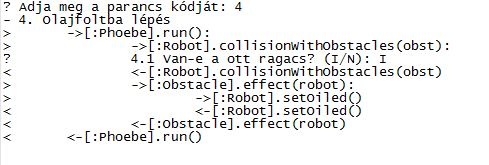
\includegraphics[width=17cm]{images/szkeleton.JPG}
\label{fig:example2}
\end{center}
\end{figure}

\pagebreak

\section{Szekvencia diagramok a belső működésre}
\subsection{Robot::CheckpointSearch}
\begin{figure}[h]
\begin{center}
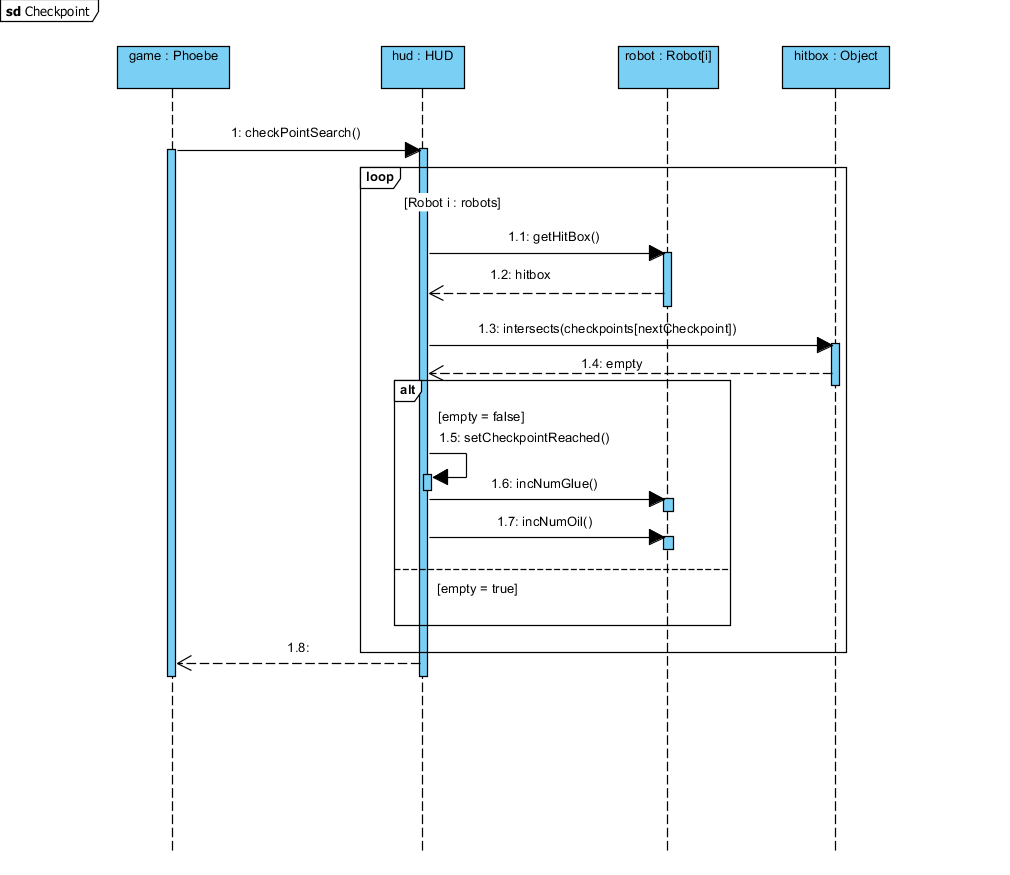
\includegraphics[width=17cm]{images/CheckpointSearch.PNG}
\caption{Következő checkpoint vizsgálata}
\label{fig:example2}
\end{center}
\end{figure}
\pagebreak

\subsection{Robot::CollisonWithObstacle}
\begin{figure}[h]
\begin{center}
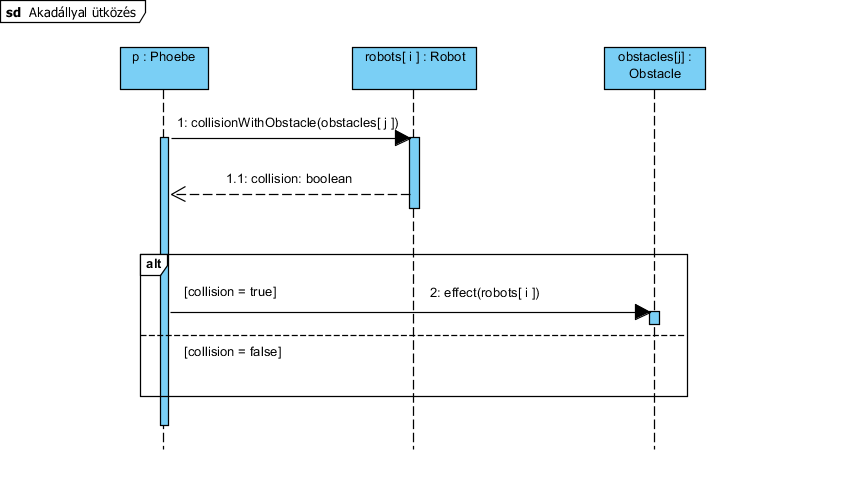
\includegraphics[width=17cm]{images/collisionWithObstacle()_sequence.PNG}
\caption{Robot ütközése akadállyal}
\label{fig:example4}
\end{center}
\end{figure}
\pagebreak

\subsection{Robot::CollisionWithRobot}
\begin{figure}[h]
\begin{center}
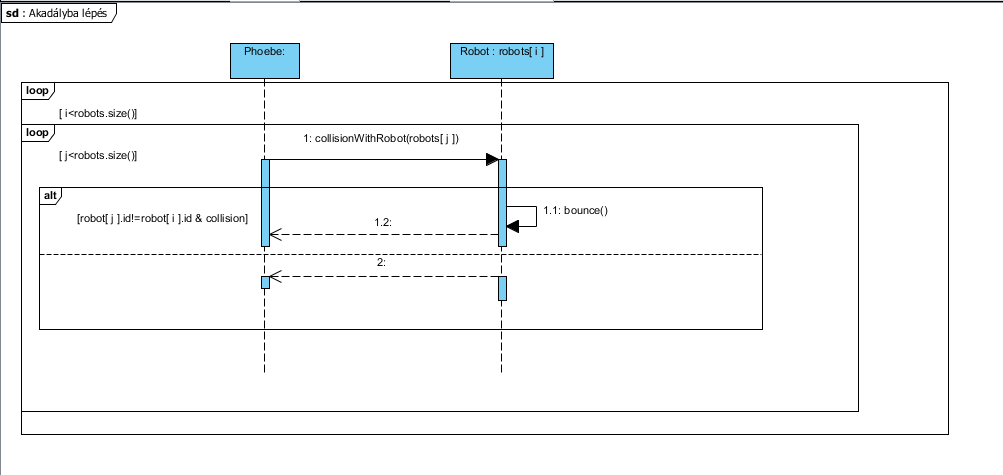
\includegraphics[width=17cm]{images/collisionWithRobot()_sequence.PNG}
\caption{Robot ütközése másik robottal}
\label{fig:example5}
\end{center}
\end{figure}
\pagebreak

\subsection{Robot::FallDown}
\begin{figure}[h]
\begin{center}
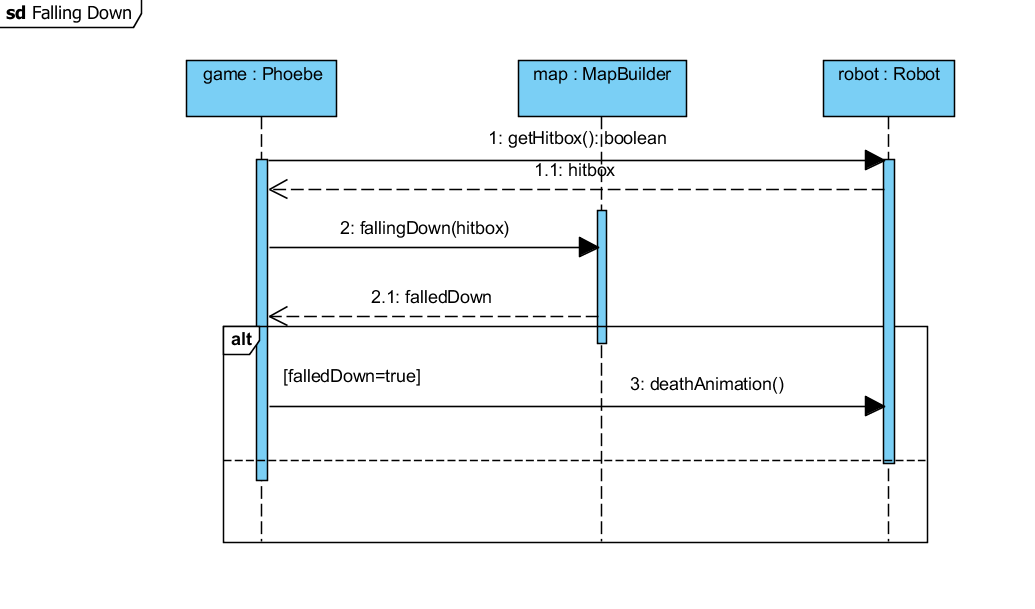
\includegraphics[width=17cm]{images/FallingDown.PNG}
\caption{Robot leesése a pályáról}
\label{fig:example6}
\end{center}
\end{figure}
\pagebreak

\subsection{Robot::InitGame}
\begin{figure}[h]
\begin{center}
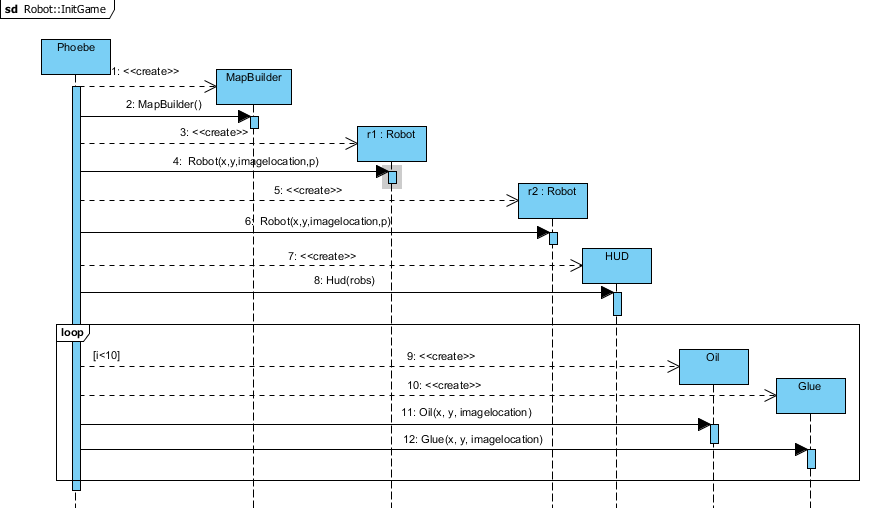
\includegraphics[width=17cm]{images/RobotInitGame.PNG}
\caption{A játék inicializálása}
\label{fig:example7}
\end{center}
\end{figure}
\pagebreak

\subsection{Robot::Move}
\begin{figure}[h]
\begin{center}
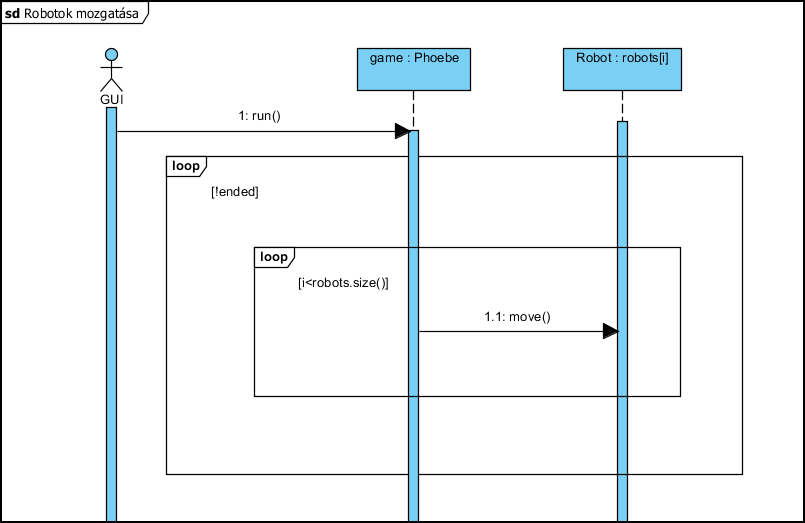
\includegraphics[width=17cm]{images/RobotMove.png}
\caption{A robot mozgatása}
\label{fig:example8}
\end{center}
\end{figure}
\pagebreak

\subsection{Robot::NewObstacle}
\begin{figure}[h]
\begin{center}
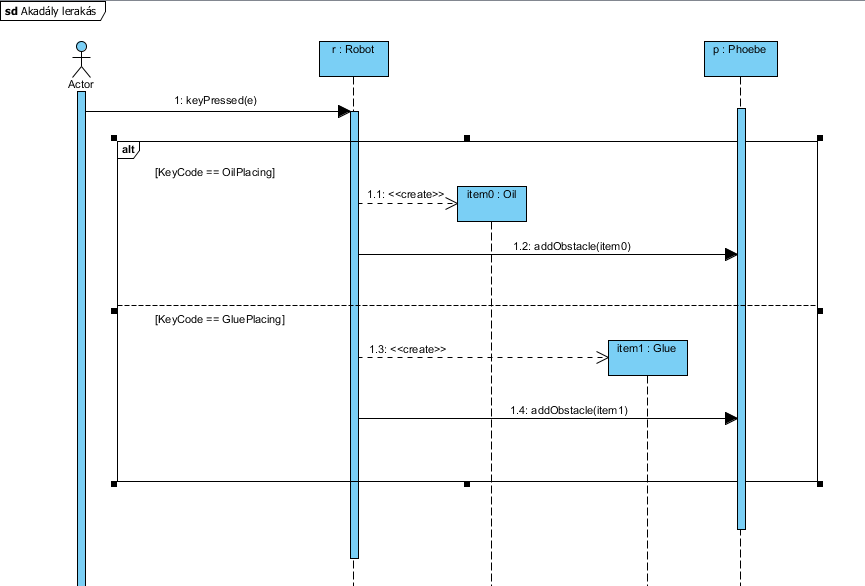
\includegraphics[width=17cm]{images/RobotAddObstacle.png}
\caption{Akadály lerakása}
\label{fig:example9}
\end{center}
\end{figure}
\pagebreak

\subsection{Robot::Settings}
\begin{figure}[h]
\begin{center}
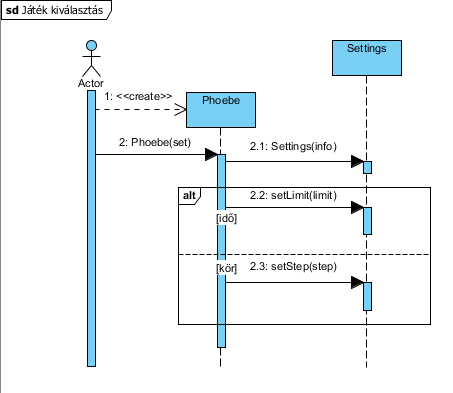
\includegraphics[width=17cm]{images/kivalasztas.PNG}
\caption{A játék beállításainak kiválasztása}
\label{fig:example10}
\end{center}
\end{figure}
\pagebreak

\subsection{Robot::End}
\begin{figure}[h]
\begin{center}
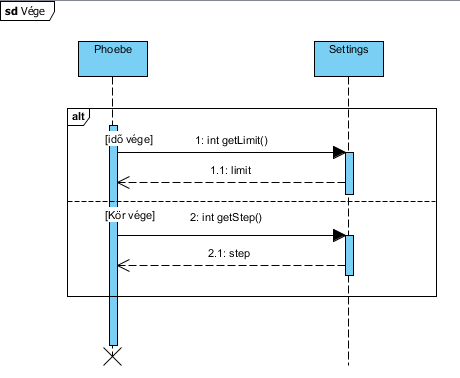
\includegraphics[width=17cm]{images/end.PNG}
\caption{Játék vége}
\label{fig:example11}
\end{center}
\end{figure}
\pagebreak

\section{Kommunikációs diagramok}

\subsection{Robot::CheckpointSearch}
\begin{figure}[h]
\begin{center}
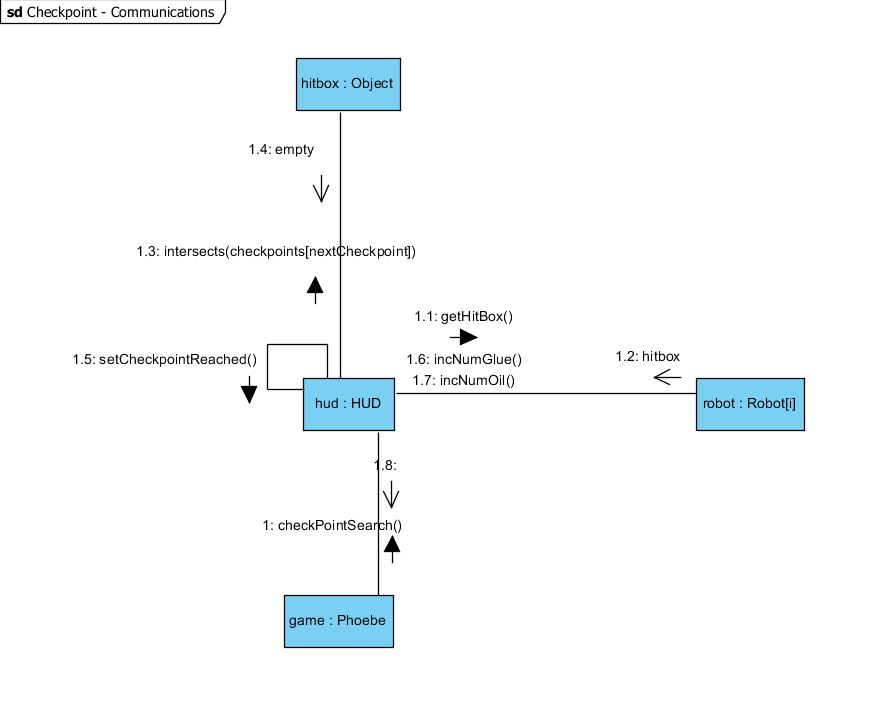
\includegraphics[width=17cm]{images/Commdiagrams/Comm_CheckpointSearch.jpg}
\caption{Következő checkpoint vizsgálata}
\label{fig:example2}
\end{center}
\end{figure}
\pagebreak

\subsection{Robot::CollisonWithObstacle}
\begin{figure}[h]
\begin{center}
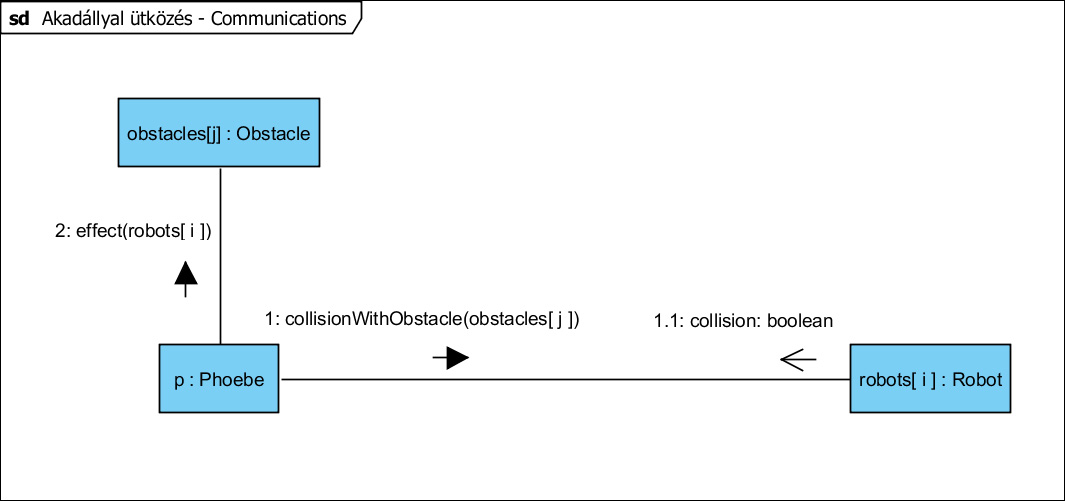
\includegraphics[width=17cm]{images/Commdiagrams/Comm_CollisionWithObstacle.jpg}
\caption{Robot ütközése akadállyal}
\label{fig:example4}
\end{center}
\end{figure}
\pagebreak

\subsection{Robot::CollisionWithRobot}
\begin{figure}[h]
\begin{center}
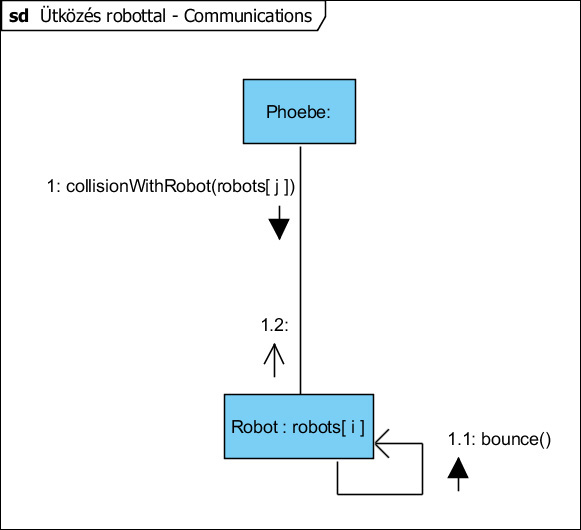
\includegraphics[width=17cm]{images/Commdiagrams/Comm_CollisionWithRobot.jpg}
\caption{Robot ütközése másik robottal}
\label{fig:example5}
\end{center}
\end{figure}
\pagebreak

\subsection{Robot::FallDown}
\begin{figure}[h]
\begin{center}
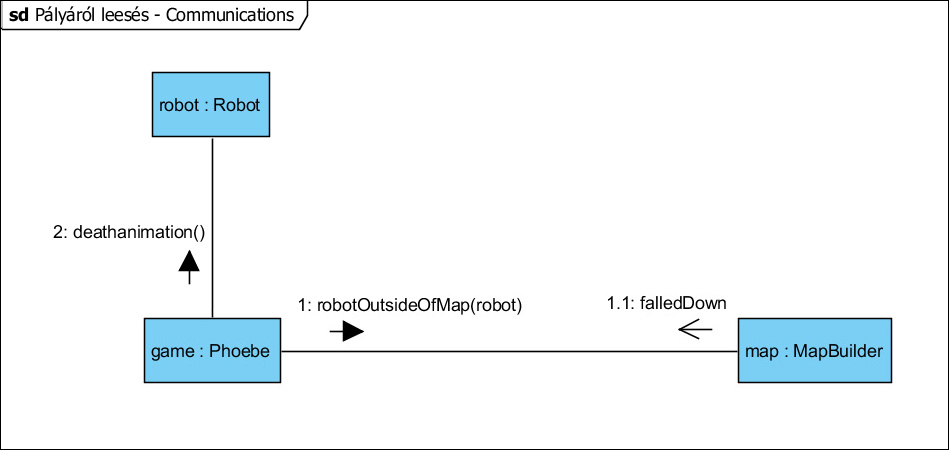
\includegraphics[width=17cm]{images/Commdiagrams/Comm_FallingDown.jpg}
\caption{Robot leesése a pályáról}
\label{fig:example6}
\end{center}
\end{figure}
\pagebreak

\subsection{Robot::InitGame}
\begin{figure}[h]
\begin{center}
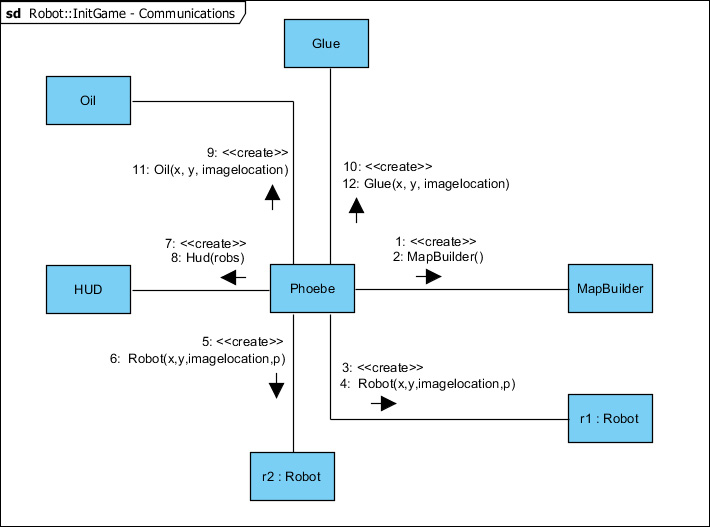
\includegraphics[width=17cm]{images/Commdiagrams/Comm_InitGame.jpg}
\caption{A játék inicializálása}
\label{fig:example7}
\end{center}
\end{figure}
\pagebreak

\subsection{Robot::Move}
\begin{figure}[h]
\begin{center}
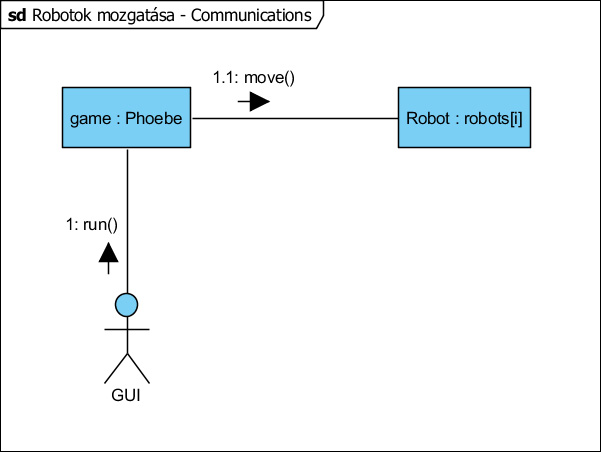
\includegraphics[width=17cm]{images/Commdiagrams/Comm_RobotMove.jpg}
\caption{A robot mozgatása}
\label{fig:example8}
\end{center}
\end{figure}
\pagebreak

\subsection{Robot::NewObstacle}
\begin{figure}[h]
\begin{center}
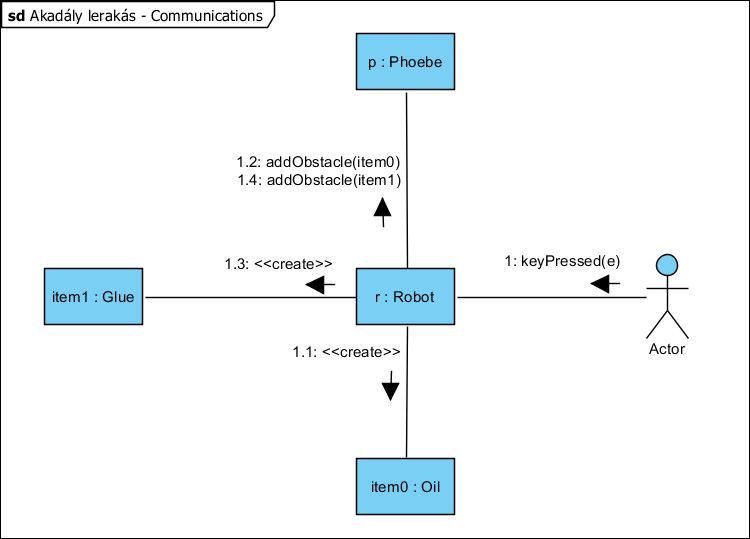
\includegraphics[width=17cm]{images/Commdiagrams/Comm_RobotAddObstacle.jpg}
\caption{Akadály lerakása}
\label{fig:example9}
\end{center}
\end{figure}
\pagebreak

\subsection{Robot::Settings}
\begin{figure}[h]
\begin{center}
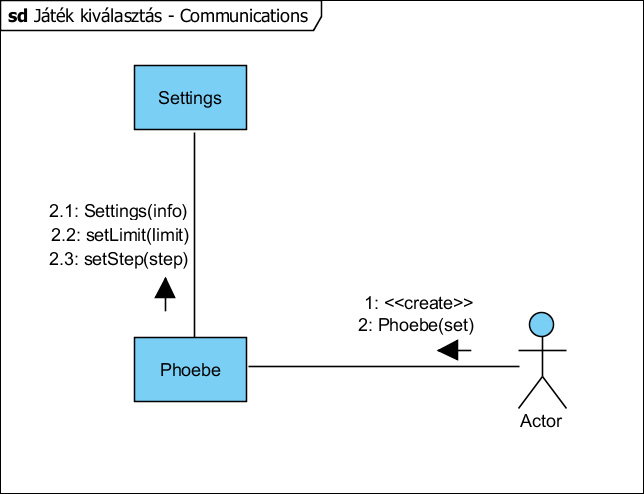
\includegraphics[width=17cm]{images/Commdiagrams/Comm_Settings.jpg}
\caption{A játék beállításainak kiválasztása}
\label{fig:example10}
\end{center}
\end{figure}
\pagebreak

\subsection{Robot::End}
\begin{figure}[h]
\begin{center}
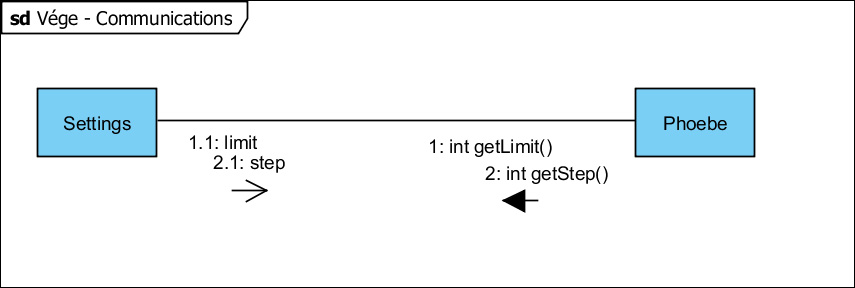
\includegraphics[width=17cm]{images/Commdiagrams/Comm_End.jpg}
\caption{Játék vége}
\label{fig:example11}
\end{center}
\end{figure}
\pagebreak